\chapter*{Introduzione}
Con HPC intendiamo ci riferiamo a \textbf{High-Performance Computing} che rappresenta il calcolo ad alte prestazioni. Il problema nasce dal fatto che, al giorno d'oggi, il computer tradizionale non basta più a causa di:
\begin{itemize}
    \item \textbf{Limiti del singolo computer}: al giorno d'oggi, i problemi sono troppo grandi per un singolo computer e un singolo computer è troppo lento.
    \item \textbf{Vincoli Sperimentali}: I problemi sono troppo costosi o impossibile da testare sperimentalmente.
    \item \textbf{Terzo pilastro}: La simulazione numerica è, piano piano, diventato un pilastro della scienza grazie al fatto che rende possibile effettuare calcoli e testare funzioni sperimentali a supporto del metodo scientifico.
    \begin{figure}[H]
        \centering
        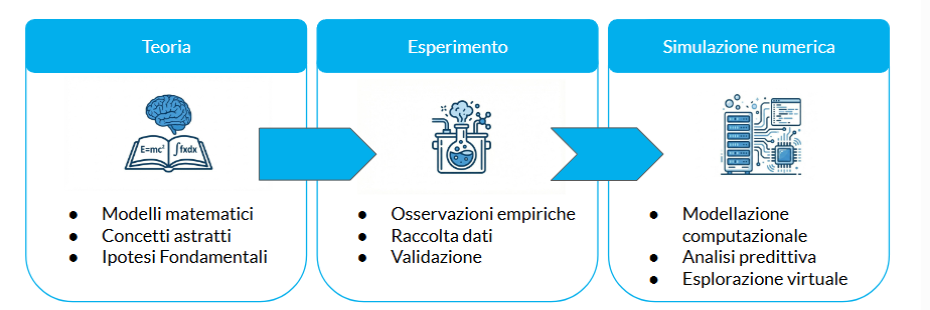
\includegraphics[width=1\linewidth]{Images/intro/metodo_sperimentale.png}
    \end{figure}
\end{itemize}

Tramite l'HPC possiamo andare a superare i problemi del calcolo sequenziale attraverso il \textbf{parallelismo} che diventa quindi una necessità strutturale a causa di quanto detto precedentemente. Infatti, quello che accade molto spesso è che i problemi hanno un fattore di crescita \textbf{non lineare} rendendo la computazione parecchio lenta nel caso in cui si aggiungano un certo numero di parametri.\\
L'\textbf{High Performance Computing (HPC)} indica l’insieme di \textbf{tecniche hardware e software} utilizzate per
risolvere problemi ad alta intensità computazionale, di memoria o di dati. Questa disciplina integra:
\begin{itemize}
    \item architetture di \textbf{calcolo parallele};
    \item \textbf{modelli di programmazione};
    \item \textbf{algoritmi e metodi numerici}.
\end{itemize}
L'obiettivo è, dunque, quello di rendere risolvibili in tempi accettabili problemi che, di norma, non lo sarebbero in un computer normale.
Le prestazioni in HPC dipendono dal corretto \textbf{bilanciamento tra hardware, software e algoritmi}.
È bene notare che il calcolo ad alte prestazioni non coincide con l’uso esclusivo di supercomputer di grandi dimensioni, bensì riguarda il modo di utilizzare le risorse sfruttando \textbf{parallelismo e gerarchia di memoria}. Le stesse tecniche HPC sono applicate infatti anche a diversi tipi di sistemi che usiamo anche quotidianamente come CPU multicore, unità vettoriali \textbf{SIMD} o acceleratori com GPU.

Il classico modello di \textbf{Von Neumann} fa delle assunzioni che sono troppo limitanti:
\begin{itemize}
    \item esecuzione di \textbf{una istruzione alla volta};
    \item un \textbf{singolo flusso di controllo};
    \item accesso a \textbf{una memoria uniforme}.
\end{itemize}
E, per quanto questo modello sia utile per descrivere algoritmi e dimostrare la loro complessità e correttezza, questa è una semplificazione troppo grossa rispetto all'hardware reale. Infatti, al giorno d'oggi il tempo di esecuzione di un programma è dominato dall'attesa dei dati in accesso dalla memoria e non dal calcolo in sé per sé. Inoltre, il modello sequenziale assume un accesso alla memoria uniforme e immediato, che non riflette la realtà.

Si può fare riferimento a due leggi:
\begin{enumerate}
    \item \textbf{Legge di Moore}:  il numero di transistor raddoppia ogni 18-24 mesi.
    \item \textbf{Scaling di Dennard}: frequenza può aumentare mantenendo potenza e dissipazione costanti migliorando l'hardware.
\end{enumerate}
Il risultato di queste due leggi è che abbiamo un aumento automatico delle prestazioni grazie a più transistor e, quindi, un' esecuzione più veloce del codice sequenziale. Tuttavia, nel 2006 lo scaling di Dennard si è arrestato e si arriva al punto in cui non si può fare meglio di così sfruttando solo codice sequenziale. È dunque necessario \textbf{sfruttare l'hardware in parallelo} e sfruttare in modo efficiente la \textbf{gerarchia di memoria}. Per cui, e prestazioni diventano una responsabilità del programmatore e si rende necessario adottare il \textbf{performance engineering}.
\begin{figure}[H]
    \centering
    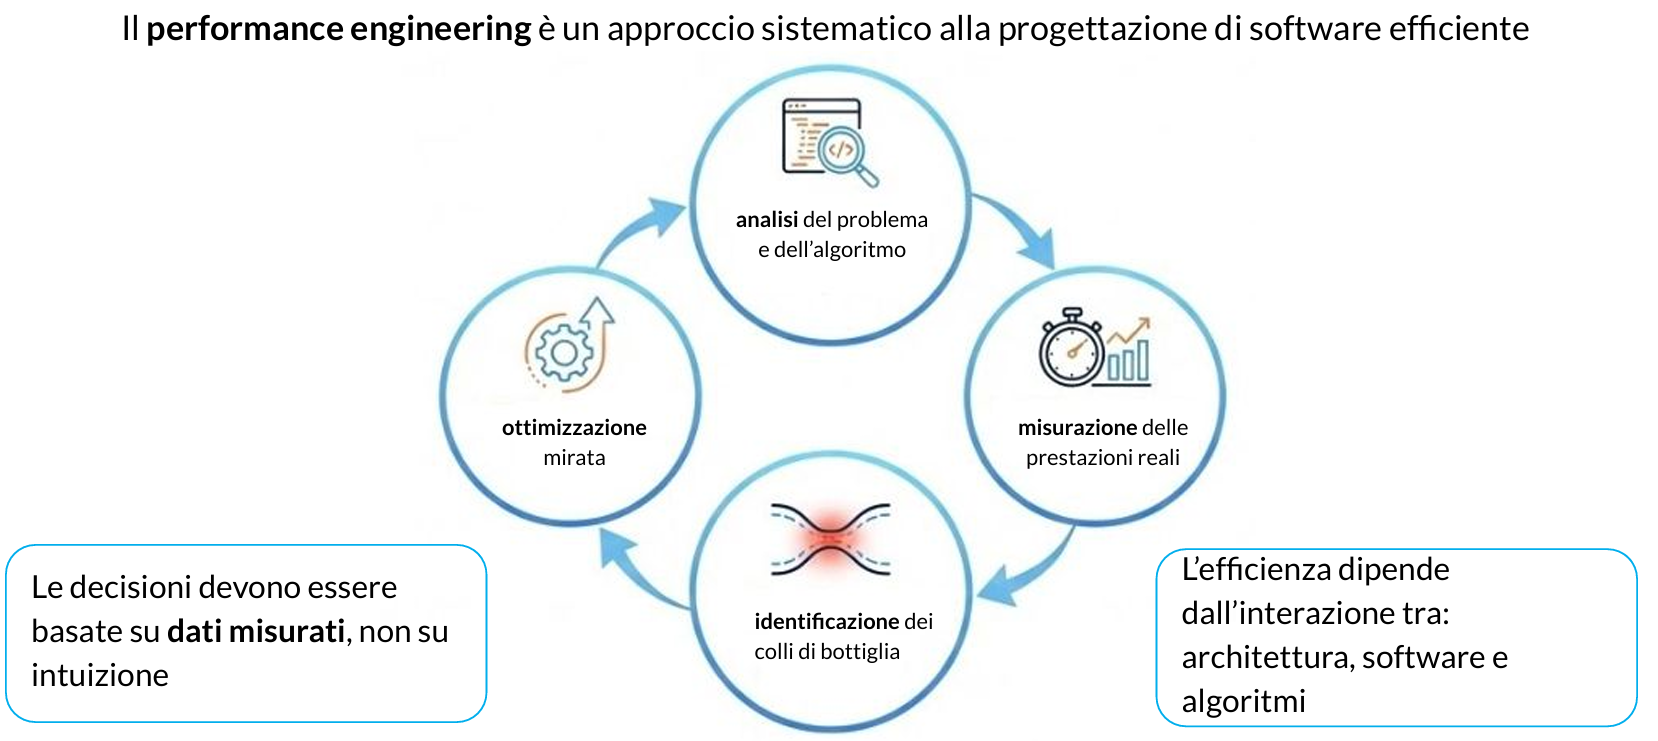
\includegraphics[width=0.85\linewidth]{Images/intro/performance_engineering.png}
\end{figure}
L’hardware moderno è intrinsecamente parallelo e sfrutta sistemi \textbf{multicore}, fa uso di \textbf{Hyper-Threading} cioè possono coesistere più thread hardware per core e sfrutta \textbf{Acceleratori GPU}. Per fruttare a pieno queste architetture, è necessario che il software sia \textbf{esplicitamente parallelo}.
Esistono più livelli di parallelismo:
\begin{enumerate}
    \item \textbf{Bit-level parallelism}: operazioni su parole di dimensione crescente;
    \item \textbf{Instruction-level parallelism (ILP)}: pipeline ed esecuzione fuori ordine;
    \item \textbf{Data-level parallelism}: operazioni vettoriali (SIMD) cioè che vengono effettuate contemporaneamente su dati diversi;
    \item \textbf{Thread-level parallelism}: esecuzione concorrente di più thread in parallelo;
    \item \textbf{Process-level parallelism}: esecuzione distribuita su più processi o nodi;
\end{enumerate}
Ogni livello contribuisce alle prestazioni complessive e ignorarne anche solo uno porta a un uso non efficiente dell’hardware.

Un sistema HPC è tipicamente organizzato come un cluster di nodi di calcolo i cui nodi sono collegati tramite una rete ad alte prestazioni a \textbf{bassa latenza e alta banda}. I dati sono spesso gestiti tramite \textbf{storage condivisi} accessibili a tutti.
Un cluster è un \textbf{insieme di nodi di calcolo indipendenti}, collegati tramite una rete ad alte prestazioni
Ogni nodo dispone di una propria CPU, memoria e acceleratori e un sistema operativo completo.
Il sistema è gestito tramite uno \textbf{stack software stratificato} che garantisce correttezza, prestazioni e scalabilità. Abbiamo diversi livelli dello stack:
\begin{itemize}
    \item \textbf{Applicazioni}: che rappresentano i codici scientifici da eseguire.
    \item \textbf{Librerie}: che sono librerie che forniscono supporto al calcolo numerico e al parallelismo.
    \item \textbf{Runtime}: ciò che gestisce l'esecuzione parallela.
    \item \textbf{Scheduler}: che alloca le risorse e gestisce i job. Nel nostro caso è bene segnalare che sfrutteremo lo scheduler SLURM che rappresenta l'attuale standard del settore.
    \item \textbf{Compilatori}: che traducono il codice in codice macchina ottimizzato per una specifica architettura.
\end{itemize}
Tra questi, un ruolo fondamentale vedremo che lo avrà lo \textbf{schedure} che si occuperà di gestire le risorse del cluster. Così facendo, gli utenti non eseguono i programmi direttamente, bensì sottomettono i job allo scheduler che li gestirà e ordinerà a seconda di quelle che sono le sue policy e delle risorse che può allocare. Questo viene fatto per far sì che sia lo scheduler a garantire l'uso efficiente delle risorse e l'equità tra gli utenti.
Come abbiamo già detto, dunque, non basterà scrivere codice corretto, abbiamo anche bisogno di \textbf{pensare in termini di parallelismo} e gestire esplicitamente dati, comunicazione e sincronizzazione.